\chapter{Introduction}
\label{chap:intro}

One can find papers with its bib on \emph{Google Scholar}.
Citation is simple~\cite{yeh2016flattened,intel_ocl_spm}, but remember that space after comma is not allowed.

Please draw figures by yourself as possible and export to pdf format, which contains words and vector graphics.
Two methods can be used to reference a figure, ex: reference the number Figure~\ref{fig:simple_figure}.
Remember the "\textasciitilde" is required to force an empty space before the referenced number.
The other way is using auto reference which generates the text for you as well, \autoref{fig:simple_figure}
If you apply auto reference on table, the text will be set to~\autoref{table:simple_table} and~\autoref{table:big_table}.

\begin{figure}[tbh!]
\centering
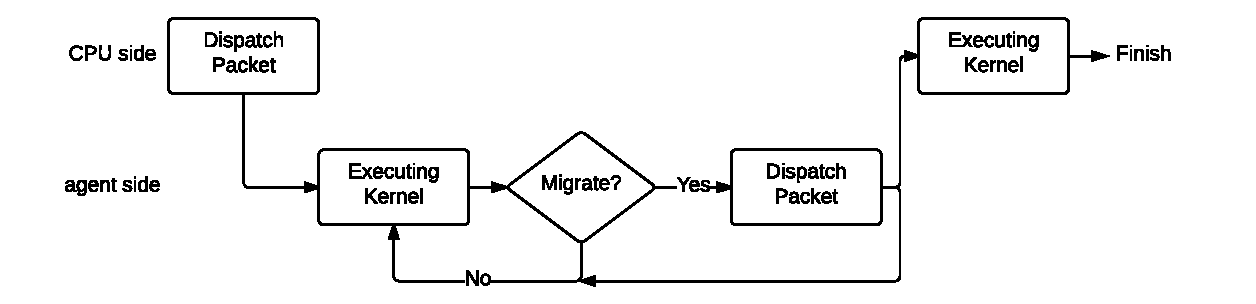
\includegraphics[width=0.95\columnwidth]{figures/flowchart}
\caption{Flow chart of something}
\label{fig:simple_figure}
\end{figure}

Tables are usually too long, we suggest to put all tables in external files.

\begin{scriptsize}
\begin{table}[tbh!]
\centering
\begin{tabular}{|c|c|c|}
\hline
Accuracy  & Recall    & Precision \\ \hline
90.556\%  & 87.0504\% & 87.6812\% \\
(337/371) & (121/139) & (121/138) \\ \hline

\end{tabular}
\caption{A simple table}
\label{table:simple_table}
\end{table}
\end{scriptsize}




% The "*" will make this table across two columns if the template is in two-column mode
\begin{table*}[tbh!]
\centering
\resizebox{\columnwidth}{!}{%
\begin{tabular}{|K{2cm}|K{2.5cm}|K{1.5cm}|K{1.5cm}|K{1.5cm}|K{1.5cm}|K{1.5cm}|K{1.5cm}|}
\hline
Metrics & Data          &   CPU  & \multicolumn{3}{c|}{Cache} & Memory & Branch    \\ \cline{4-6}
        & Structure     &         & L1I     & L1D     & L2D   &        &           \\ \hline
\multirow{2}{*}{\begin{minipage}{2cm}\centering Miss Rate\end{minipage}}
        & Ordered Map   & -       & 0.000   & 0.019   & 0.247 & -      & 0.100     \\
        & Unordered Map & -       & 0.000   & 0.036   & 0.305 & -      & 0.089     \\ \hline

\multirow{2}{*}{\begin{minipage}{2cm}\centering Access Times\end{minipage}}
        & Ordered Map   & 863.04M & 231.36M & 491.50M & 9.92M & 2.45M  & 194.30M   \\
        & Unordered Map & 310.33M & 70.57M  & 81.46M  & 3.38M & 1.03M  & 44.34M    \\ \hline

\multirow{2}{*}{\begin{minipage}{2cm}\centering Estimated Time(s)\end{minipage}}
        & Ordered Map   & 0.174s  & \multicolumn{3}{c|}{0.790s} & 0.270s  & 0.325s \\
        & Unordered Map & 0.126s  & \multicolumn{3}{c|}{0.230s} & 0.190s  & 0.066s \\ \hline

\end{tabular}
}
\caption[Performance breakdown of data structures]
{Performance-counter comparison and breakdown of the Program ID 16 (A Map) and Program ID 20 (B Map)}
\label{table:big_table}
\end{table*}



Codes can be written/colored in two ways.
Listing~\autoref{fig:code_wordcount} and Minted~\autoref{fig:code_wordcount_minted}.
Usually, \emph{listing} is more prefered because the results from \emph{minted} is \textbf{too fancy}.
In addition, \emph{minted} takes more time to prcess and generates \emph{\_minted-*} directory.

\begin{figure}[tbh!]
\begin{lstlisting}{c++}
void create_map(auto &str_map, auto &str_vector) {
    // Iterate through str_vector
    for (auto &&v : str_vector) {
        // Accumulate
        str_map[v] += 1;
    }
}
\end{lstlisting}
\caption[Code of Wordcount with Listing]
{Code for spliting spaces and building a word count map in C++14.}
\label{fig:code_wordcount}
\end{figure}

\begin{figure}[tbh!]
\begin{minted}{c++}
void create_map(auto &str_map, auto &str_vector) {
    // Iterate through str_vector
    for (auto &&v : str_vector) {
        // Accumulate
        str_map[v] += 1;
    }
}
\end{minted}
\caption[Code of Wordcount with Minted]
{Code for spliting spaces and building a word count map in C++14.}
\label{fig:code_wordcount_minted}
\end{figure}



Algorithm in pseudo code can be written as demoed in \autoref{alg:simple_algorithm}.

\begin{algorithm} % enter the algorithm environment
\caption{How to write algorithms}
\begin{algorithmic}
\If {$i\geq maxval$}
    \State $i\gets 0$
\Else
    \If {$i+k\leq maxval$}
        \State $i\gets i+k$
    \EndIf
\EndIf
\end{algorithmic}
\label{alg:simple_algorithm}
\end{algorithm}


HTML output can be done by \emph{make html} command.
One can use this to generate text, i.e. list of figures and bibliography, for copying to website when submitting thesis.

